\section{Zielsetzung}
\label{sec:Zielsetzung}
Ziel des Versuches ist es, die mittlere Lebensdauer von kosmischen Myonen mittels eines Szintillationsdetektors zu bestimmen. 

\section{Theorie}
\label{sec:Theorie}
\subsection{Eigenschaften und Entstehung kosmischer Myonen}
Myonen, $\mu$, sind Elementarteilchen des Standardmodells der Teilchenphysik. Sie gehören zu der Familie der Leptonen und werden zusammen mit ihrem zugehörigen Neutrino $\nu_\mu$ in der zweiten Generation eingeordnet \ref{fig:std}.
\begin{figure}[H]
    \centering
    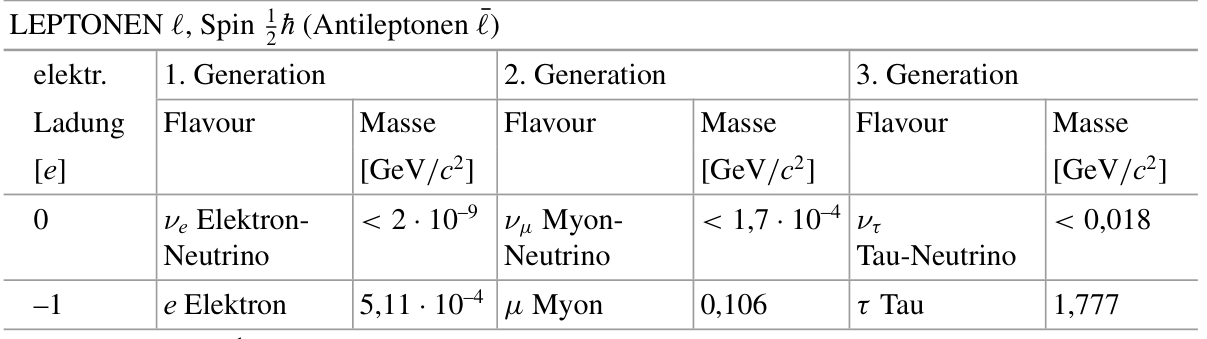
\includegraphics[width=\linewidth]{data/leptonen_std.png}
    \captionof{figure}{Die drei Leptonengenerationen des Standardmodells \cite{astro}}
    \label{fig:std}
\end{figure}
\noindent
Myonen haben Spin $\frac{1}{2}$ und sind daher Fermionen. Sie haben eine negative Ladung von $q = \SI{-1}{e}$ und wiegen mit $m_\mu \approx \SI{106}{MeV}$ ca. $200$ mal so viel wie ein Elektron mit $m_e \approx \SI{0.511}{keV}$. Die in diesem Versuch zu bestimmende mittlere Lebensdauer der Myonen beträgt $\tau_{\mu} = \SI{2.2}{\micro\second}$ \cite{pdg}, diese Zerfallen zu ca. 100\% \cite{pdg} über ein $W^{-}$ Boson in ein Elektron und zwei Neutrinos, nach 
\begin{equation}
    \mu^- \rightarrow e^- + \bar{\nu}_e + \nu_\mu
\end{equation}
Kosmische Myonen entstehen in einer höhe von ca. $\SI{20}{km}$ in sogenannten Luftschauern. Diese finden statt, wenn ein hochenergetisches Teilchen aus dem kosmos auf die Erdatmosphäre trifft und dort mit den Teilchen dieser wechselwirkt.
Bei nicht zu hohen Energien sind Protonen die häufigsten Primärteilchen. Diese Treffen auf die Atmosphäre und zerfallen bei der Wechselwirkung mit den Atomen und Molekülen der Erdatmosphäre in Kaonen und Pionen. Kaonen und Pionen zerfallen weiter in Myonen, wie hier Beispielhaft für $K^-$ und $\pi^-$ nach
\begin{equation}
    \begin{aligned}
        K^- &\rightarrow \mu^- &+ \bar{\nu}_\mu \\
        \pi^- &\rightarrow \mu^- &+ \bar{\nu}_\mu
    \end{aligned}
\end{equation}
welche als häufigstes Teilchen auf Meereshöhe gemessen werden.
\begin{figure}[H]
 \centering
 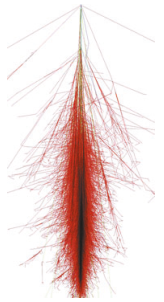
\includegraphics[width=0.2\linewidth]{data/Luftschauer.png}
 \captionof{figure}{Simulation eines Luftschauers, ausgelöst durch ein kosmisches Proton bei $E_p = \SI{1}{TeV}$ \cite{astro}}
 \label{fig:luftschauer}
\end{figure}
\noindent
Grund für das erreichen des Bodens der Myonen sind relativistische Effekte. Ein Myon mit einer Energie von $E_{\mu} = \SI{10}{GeV}$ fliegt nach 
\begin{equation}
    \label{eqn:t1}
    v_\mu = \frac{\frac{p_\mu}{m_\mu}}{\sqrt{1 + \left( \frac{p_\mu}{m_\mu} \right)^{2}}}
\end{equation}
mit einer Geschwindigkeit von ca. $v_{\mu} \approx 0.9999 \cdot \symup{c}$, wobei sich $p_\mu$ durch 
\begin{equation}
    p_\mu = \sqrt{E_\mu^2 - m_\mu^2}
\end{equation}
berechnen lässt.
Ein Teilchen mit dieser Geschwindigkeit hat somit einen Gamma Faktor von $\gamma_\mu \approx 90$. Bei einer mittleren Lebensdauer von $\tau_{\mu} = \SI{2.2}{\micro\second}$ \cite{pdg} berechnet sich die aus dem ruhendem System auf der Erdoberfläche zurückgelegte mittlere Strecke des Myons dann nach 
\begin{equation}
    \label{eqn:t2}
    s = v_{\mu} \cdot \tau_{\mu} \cdot \gamma_{\mu}
\end{equation}
auf $s \approx \SI{60000}{m}$. Bei einer klassischen Rechnung beträgt dieser Wert $s_{\symup{klassisch}} \approx \SI{650}{m}$.
\subsection{Zerfallsgesetz und mittlere Lebensdauer}
Die mittlere Lebensdauer eines Myons lässt sich aus dem Zerfallsgesetz 
\begin{equation}
    \label{eqn:t3}
    \symup{d}N = - \lambda N \symup{d}t
\end{equation}
herleiten. Dieses besagt, dass die Änderung der Anzahl an Teilchen $N$ um $\symup{d}N$ antiproportional ist zu einer Konstante $\lambda$ mal der Anzahl der Teilchen $N$ im Zeitintervall $\symup{d}t$. Aus dieser Differentialgleichung folgt, dass die Menge $N$ der nach der Zeit $t$ noch vorhandenen Teilchen der Funktion
\begin{equation}
    \label{eqn:t4}
    N\left(t\right) = N_0 \cdot \symup{exp} \left( -\lambda t \right)
\end{equation}
folgt. Dabei ist $N_0$ die Anzahl der Teilchen bei $t = 0$. Für den Fall, dass $N_0 = 1$ ist, also dass wir ein Teilchen betrachten, betrachten wir eine Verteilungsfunktion der Form 
\begin{equation}
    \label{eqn:t5}
    P\left(t\right) = \symup{exp} \left( -\lambda t \right) .
\end{equation}
Gleichung \ref{eqn:t5} gibt dabei die Wahrscheinlichkeit an, dass das betrachtete Teilchen nach der Zeit t noch nicht Zerfallen ist. Die Funktion $P\left(t\right)$ impliziert so die existenz einer Wahrscheinlichkeitsdichte der Form
\begin{equation}
    \label{eqn:t6}
    p\left(t\right) = \lambda \cdot \symup{exp} \left( -\lambda t \right) 
\end{equation}
wobei der Zusammenhang $\symup{d}P\left(t\right) = p \left(t\right) \symup{d}t$ gilt.
Die Wahrscheinlichkeitsdichte aus Gleichung \ref{eqn:t6} bedingt den Erwartungswert
\begin{equation}
    \label{eqn:t7}
    \langle t \rangle  = \int_0^{\infty} t \cdot p\left(t\right) \symup{d}t = \frac{1}{\lambda}
\end{equation}
welcher als mittlere Lebensdauer $\tau$ identifiziert wird. Es gilt daher 
\begin{equation}
    \label{eqn:t8}
    \tau = \frac{1}{\lambda}
\end{equation}
\subsection{Messprozess der kosmischen Myonen}
\newpage
\section{Versuchsaufbau}
In \autoref{fig:aufb} 
\begin{figure}[H]
    \centering
    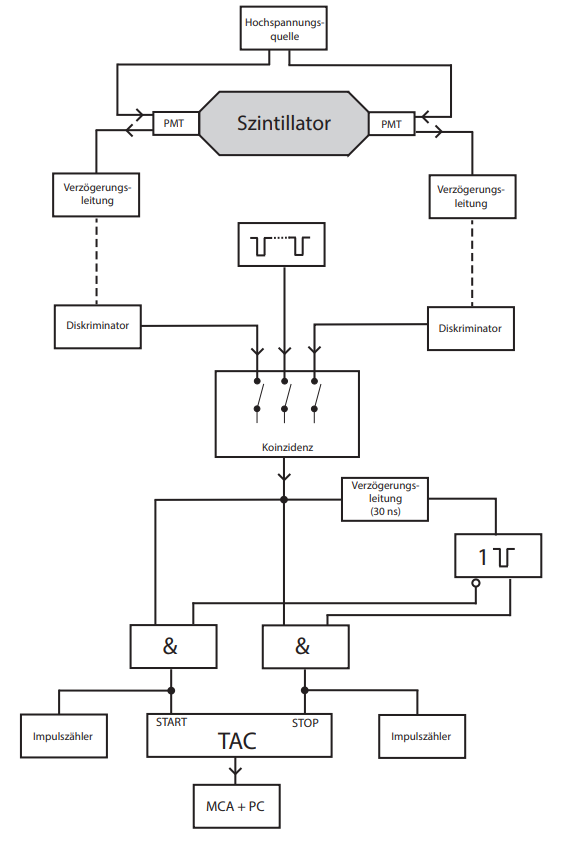
\includegraphics[width=0.6\linewidth]{data/aufbau_schem.png}
    \captionof{figure}{Schematischer Versuchsaufbau \cite{V01}}
    \label{fig:aufb}
\end{figure}
\noindent
\newpage
